\documentclass[11pt]{article}

\usepackage[utf8]{inputenc}
\usepackage[T1]{fontenc}
\usepackage{lmodern}
% \usepackage[frenchb]{babel}
\usepackage{setspace}

\usepackage{microtype}
\usepackage{mathtools}

\usepackage{subcaption}
\usepackage{graphicx}
\usepackage[bookmarks=true]{hyperref}
\usepackage{float}
\usepackage[export]{adjustbox}
\usepackage[stable]{footmisc}


\newcommand{\HRule}{\rule{\linewidth}{0.5mm}}
% \usepackage[a4paper, total={6in, 8in}]{geometry}
\usepackage{geometry}
\usepackage[numbers,sort]{natbib}
% \usepackage[nocompress]{cite}
\geometry{a4paper,top=2.54cm,bottom=2.54cm,left=2.54cm,right=2.54cm,heightrounded}
% \geometry{top=0.1cm,bottom=0.1cm,left=0.9cm,right=0.9cm}
\usepackage{pdfpages}
\usepackage{listings}
\usepackage{color}
\usepackage{multirow}
\usepackage{hyperref}

\usepackage{pdfpages}
\usepackage{listings}
\usepackage{color}
\usepackage{multirow}
\usepackage{hyperref}
\usepackage{amsfonts}
\usepackage{amssymb}
\usepackage{mathrsfs}
\usepackage{authblk}
\usepackage{bbm}
\usepackage{multirow}
\usepackage{float}
\floatstyle{plaintop}
\restylefloat{table}
\usepackage[algoruled,boxed,lined]{algorithm2e}
% linesnumbered,
\usepackage{chngcntr}
\counterwithout{algocf}{section}
% \counterwithin*{algocf}{subsection}
% \counterwithin*{algocf}{subsubsection}
% \renewcommand{\thealgocf}{\arabic{section}.\arabic{subsection}.\arabic{subsubsection}.\arabic{algocf}}
\renewcommand{\thealgocf}{\arabic{section}.\arabic{algocf}}
\usepackage{tabulary}
\usepackage{tabularx}

\numberwithin{equation}{section}
% \numberwithin{equation}{subsection}
% \numberwithin{equation}{subsubsection}

\usepackage{chngcntr}
\counterwithin{table}{section}
% \counterwithin{table}{subsection}
% \counterwithin{table}{subsubsection}

\counterwithin{figure}{section}
% \counterwithin{figure}{subsection}
% \counterwithin{figure}{subsubsection}

\definecolor{codegreen}{rgb}{0,0.6,0}
\definecolor{codegray}{rgb}{0.5,0.5,0.5}
\definecolor{codepurple}{rgb}{0.58,0,0.82}
\definecolor{backcolour}{rgb}{0.95,0.95,0.92}
 
\lstdefinestyle{mystyle}{
    backgroundcolor=\color{backcolour},   
    commentstyle=\color{codegreen},
    keywordstyle=\color{magenta},
    numberstyle=\tiny\color{codegray},
    stringstyle=\color{codepurple},
    basicstyle=\footnotesize,
    breakatwhitespace=false,         
    breaklines=true,                 
    captionpos=b,                    
    keepspaces=true,                 
    numbers=left,                    
    numbersep=5pt,                  
    showspaces=false,                
    showstringspaces=false,
    showtabs=false,                  
    tabsize=2
}
 
\lstset{style=mystyle}
\DeclareUnicodeCharacter{00A0}{ }

\setlength{\parindent}{0pt}
\setlength{\parskip}{10pt plus 5pt minus 3pt}

\hypersetup{
unicode=false,          % non-Latin characters in Acrobat’s bookmarks
colorlinks=true,        % false: boxed links; true: colored links
linkcolor=black,        % color of internal links (change box color with linkbordercolor)
citecolor=blue,        % color of links to bibliography
filecolor=magenta,      % color of file links
urlcolor=blue}           % color of external links

\newcommand*{\SuperScriptSameStyle}[1]{%
  \ensuremath{%
    \mathchoice
      {{}^{\displaystyle #1}}%
      {{}^{\textstyle #1}}%
      {{}^{\scriptstyle #1}}%
      {{}^{\scriptscriptstyle #1}}%
  }%
}
\newcommand*{\oneS}{\SuperScriptSameStyle{*}}
\newcommand*{\twoS}{\SuperScriptSameStyle{**}}
\newcommand*{\threeS}{\SuperScriptSameStyle{*{*}*}}

% \usepackage[utf8]{inputenc}
% \usepackage{fourier} 
% \usepackage{array}
% \usepackage{makecell}

% \renewcommand\theadalign{bc}
% \renewcommand\theadfont{\bfseries}
% \renewcommand\theadgape{\Gape[4pt]}
% \renewcommand\cellgape{\Gape[4pt]}

% \usepackage{array}
% \newcolumntype{Z}{>{\centering\let\newline\\\arraybackslash\hspace{0pt}}X}

\usepackage[flushleft]{threeparttable}


\begin{document}
% \begin{spacing}{1}
%----------------------------------------------------------------------------------------
%   Title Page
%----------------------------------------------------------------------------------------
\pagenumbering{Alph}
\begin{titlepage}            
    \begin{flushleft}{
        \includegraphics[width=0.3\linewidth]{figures/qmul_logo.png}\\
        School of Business and Management\\
        Queen Mary University of London\\[1cm]
        Progression Paper for PhD Programme\\
        21 June 2018\\[2cm]
    }\end{flushleft}
    \centering
    \HRule \\[1cm]
    {\huge Title}\\[1cm]
    \HRule \\[1cm]

    \begin{flushleft}{
        PhD Student: \\
        PhD Supervisors: \\
        Progression Panel: \\[1cm]
    }\end{flushleft}
\end{titlepage}


\pagenumbering{arabic}
%----------------------------------------------------------------------------------------
%   Introduction
%----------------------------------------------------------------------------------------
\section{Introduction\label{sec:introduction}}

%----------------------------------------------------------------------------------------
%   Section: Literature review
%----------------------------------------------------------------------------------------
\section{Literature review\label{sec:literature_review}}

%----------------------------------------------------------------------------------------
%   Section: Data
%----------------------------------------------------------------------------------------
\section{Data\label{sec:data}}

\begin{figure}[H]
    \centering
    \begin{subfigure}[c]{.45\textwidth}
        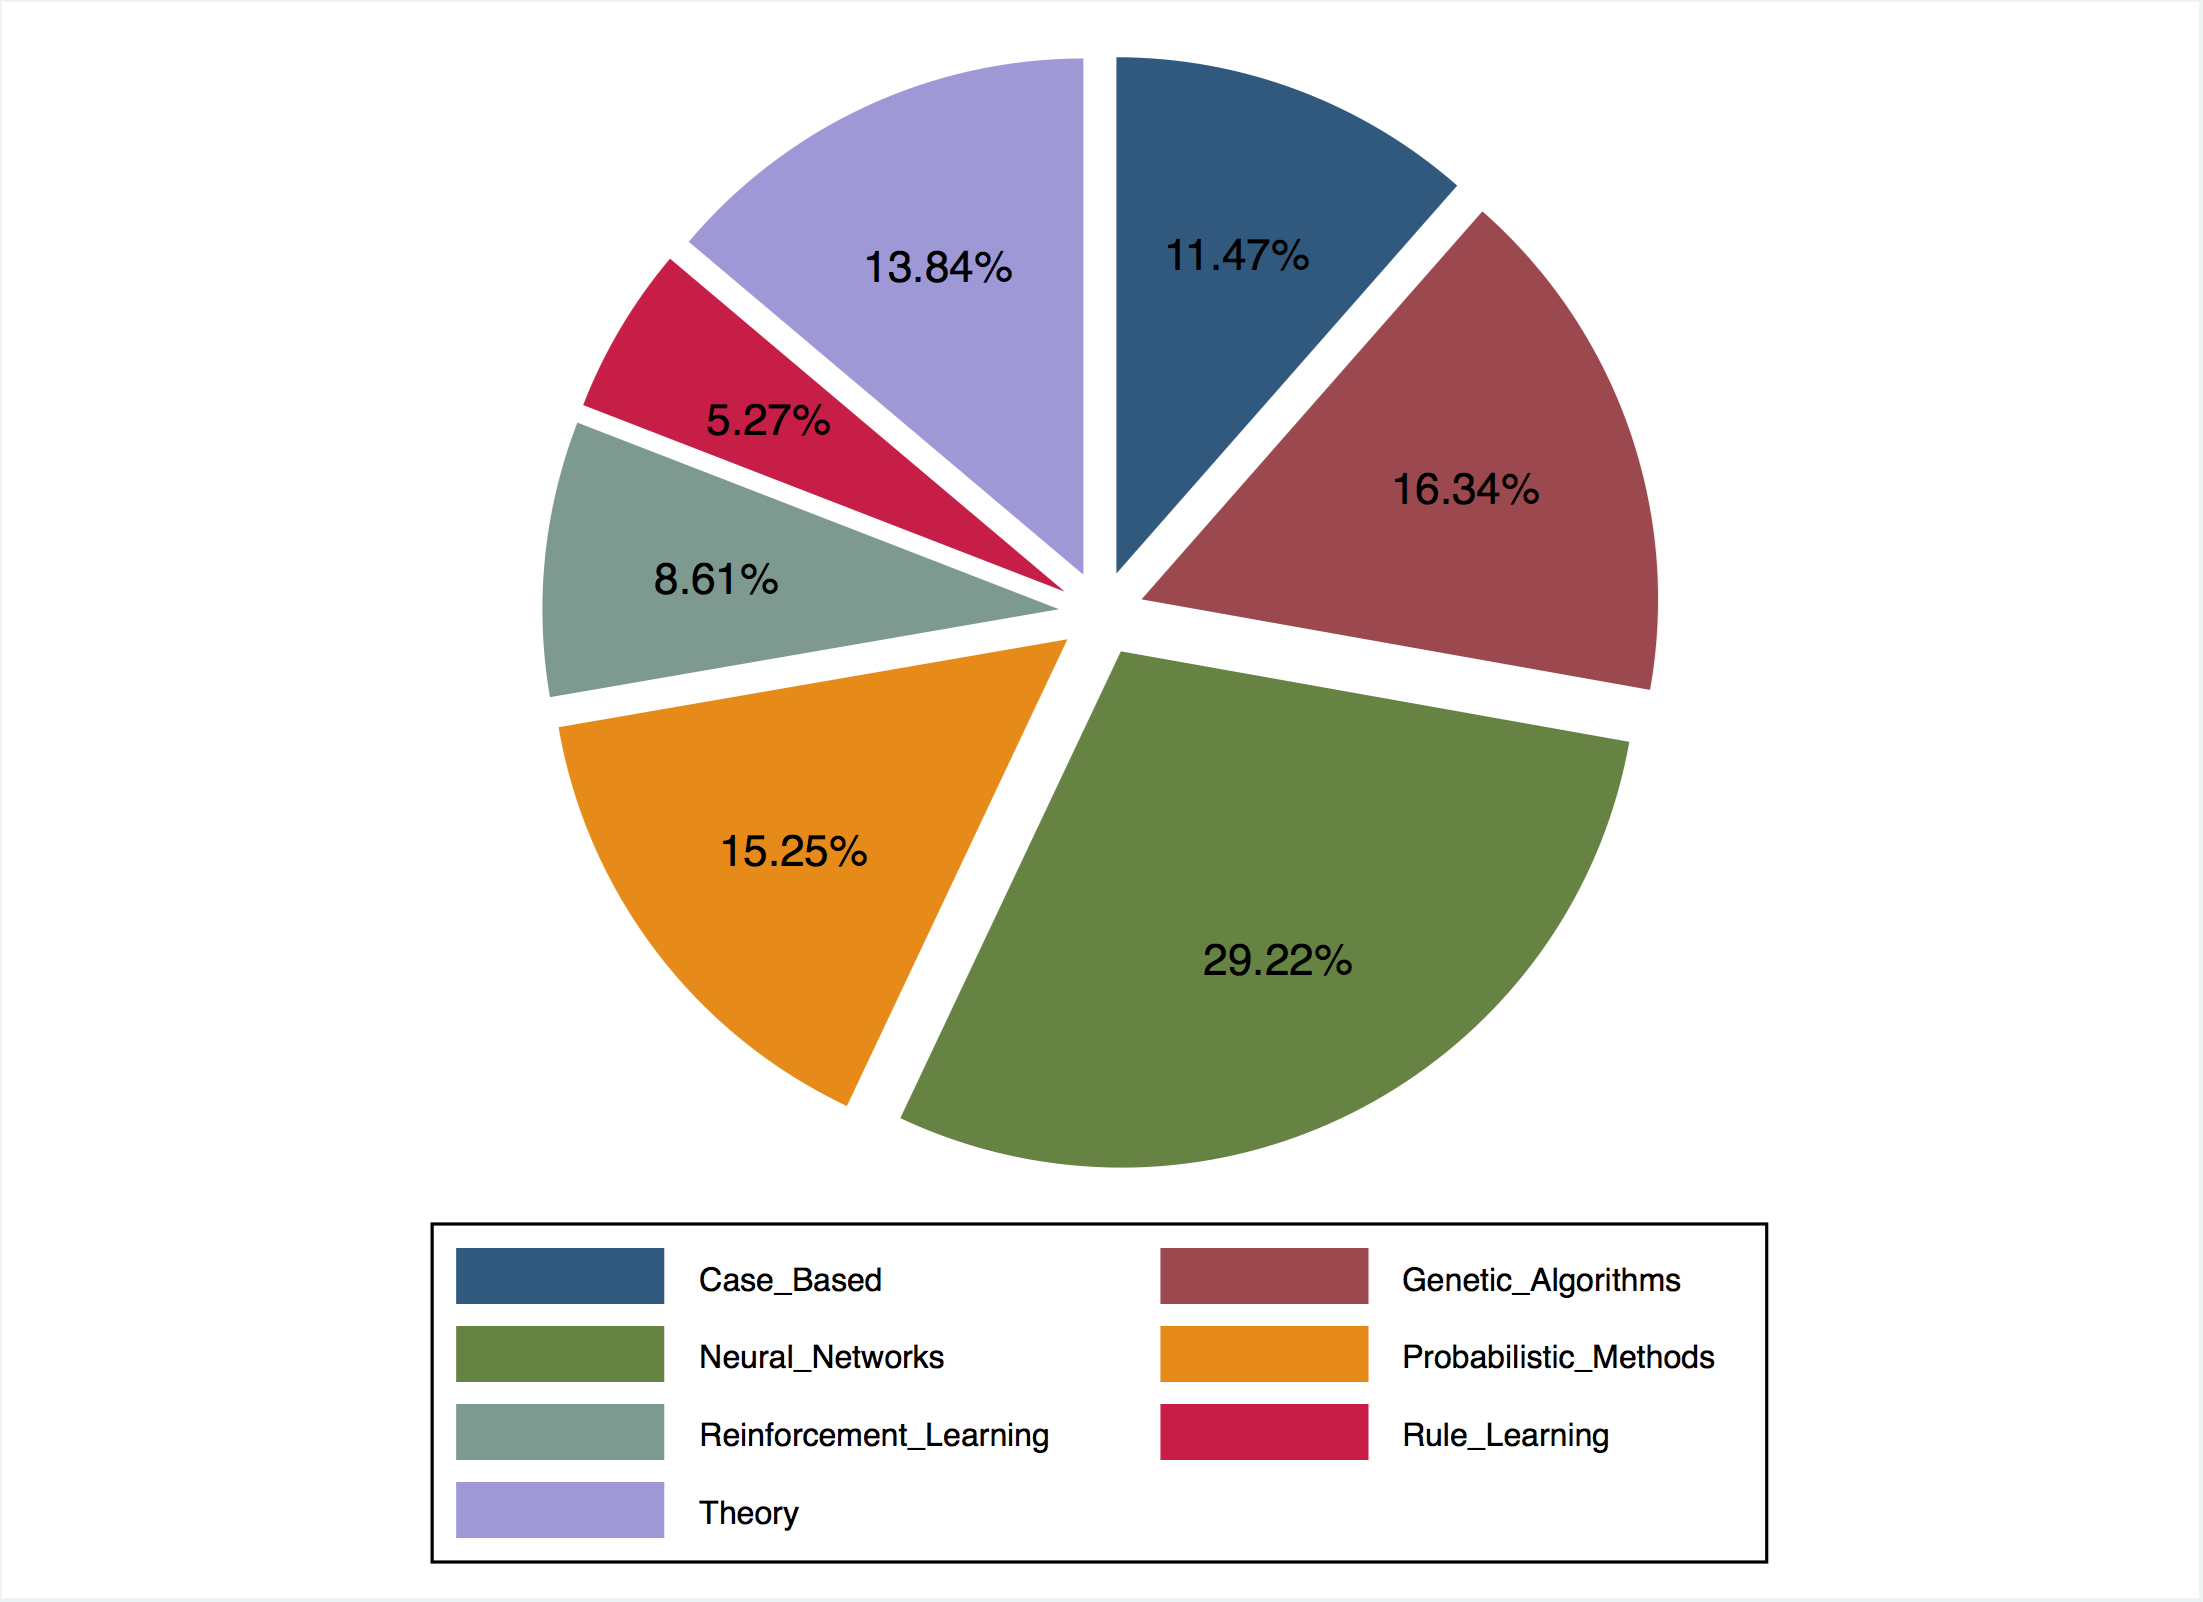
\includegraphics[width=1.0\textwidth]{figures/cora_categoriesPercent_piechart.png}
        \caption{CORA}
        \label{fig:cora_catPercent}
    \end{subfigure}
    \begin{subfigure}[c]{.45\textwidth}
        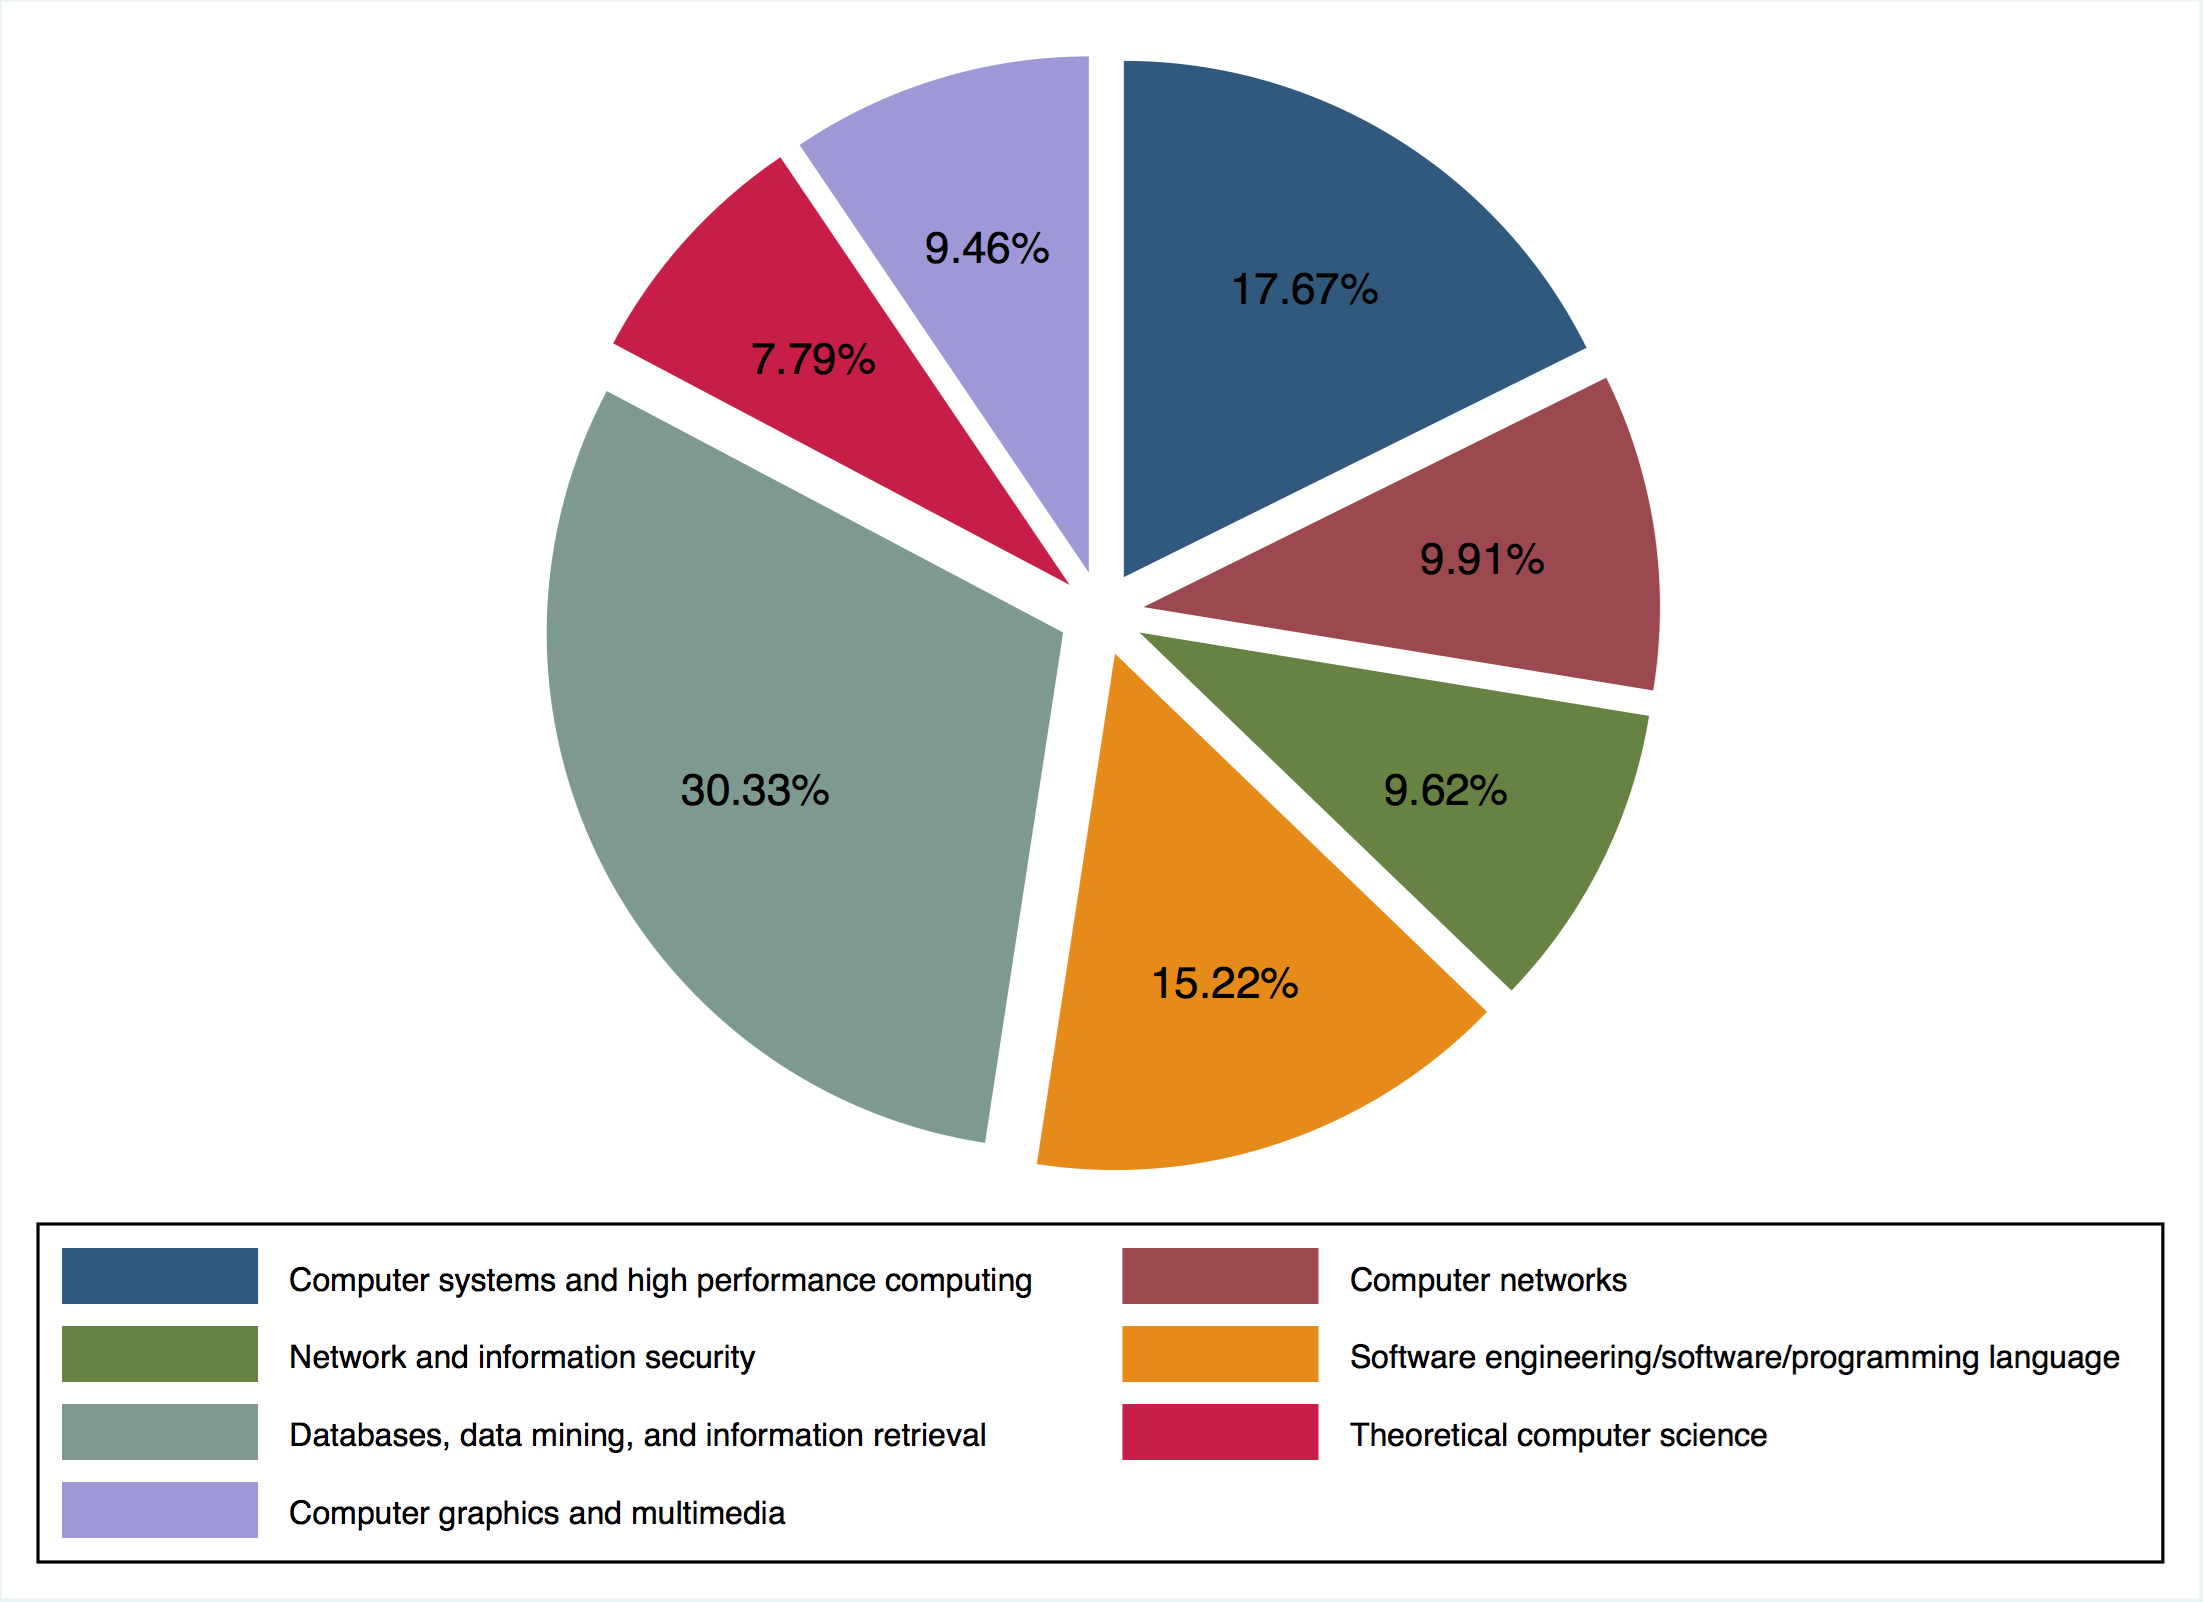
\includegraphics[width=1.0\textwidth]{figures/aminer_categoriesPercent_piechart.png}
        \caption{AMiner}
        \label{fig:aminer_catPercent}
    \end{subfigure}
    \caption{Frequency distributions of paper categories in CORA and AMiner.}
    \label{fig:dataset_catPercent}
\end{figure}
%----------------------------------------------------------------------------------------
%   Section: Research design
%----------------------------------------------------------------------------------------
\section{Methods\label{sec:research_design}}
\begin{table}[H]
    \centering
    \begin{tabular}{ c|c }
        \hline
        \textbf{Measure} & \textbf{Note} \\ \hline
        nb\_friends\_treated &  number of treated friends\\
        nb\_friends\_unTreated & number of untreated friends\\
        number\_friends\_nonEligible & number of non-eligible friends\\
        nb\_friends\_eligible & this is the sum of treated and untreated friends\\
        nb\_friends\_eligible\_and\_nonEligible & this is total sum of friends\\
        \hline
    \end{tabular}
    \caption{Measures for the students' social network - Set of number of friends~\cite{newman2010}}
    \label{table:social_network_measures_1}
\end{table}
%----------------------------------------------------------------------------------------
%   Section: Results
%----------------------------------------------------------------------------------------
\section{Results\label{sec:results}}

%----------------------------------------------------------------------------------------
%   Future work
%----------------------------------------------------------------------------------------    
\section{Conclusion and future work\label{sec:conclusion_future_work}}

%----------------------------------------------------------------------------------------
%   Achievement
%----------------------------------------------------------------------------------------    
\section{Achievement}

%----------------------------------------------------------------------------------------
%   References
%----------------------------------------------------------------------------------------
\bibliographystyle{apa}
\bibliography{references}

% \end{spacing}
\end{document}